\section{Grundlagen} \label{grundlagenKapitel}
\subsection{Aufbau des \acl{ebuef}s}
Das \ac{ebuef} ist in ein eingleisiges nicht-elektrifiziertes und ein zweigleisiges elektrifiziertes Streckennetz unterteilt, welche über die Betriebsstelle Leopoldsgrün (XLG) miteinander verbunden sind. In der Abbildung \ref{fig:ebuefNetz} wird das eingleisige Netz schwarz und die zweigleisige Hauptstrecke rot dargestellt.
\begin{figure}
  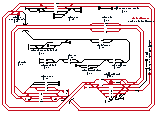
\includegraphics[width=\linewidth]{../images/netz/plan.pdf}
  \caption[Schienennetz des \ac{ebuef}s]{Schienennetz des \ac{ebuef}s (Quelle: www.ebuef.de/das-betriebs\-feld/stell\-werke; Letzter Zugriff am: 4. September 2021)}
  \label{fig:ebuefNetz}
\end{figure}
Das eingleisige Netz ist in \acp{infra}, welche mit Blockstrecken vergleichbar sind und eine Zugfolge im festen Raumabstand ermöglichen, eingeteilt.\footnote{\citet[S. 7, 42]{pachl1999systemtechnik}} Die \acp{infra} sind mit der RailCom-Technik ausgestattet, welche über Decoder in den Fahrzeugen den aktuellen \ac{infra} ermittelt und diesen in der \textit{fma}-Tabelle der \textit{MySQL}-Datenbank speichert.\footnote{\cite{railcomnorm}} Zudem sind in der Datenbank alle Informationen über die Infrastruktur gespeichert. Für die Fahrzeugsteuerung essenziell sind dabei die aktuellen Signalbegriffe aller Signale und die Längen der \acp{infra}.\footnote{\cite{ebuef}}

Der Betrieb des \ac{ebuef}s erfordert eine angelegte Session, welche vor dem Start der Fahrzeugsteuerung gestartet werden muss, da die Fahrzeugsteuerung beim Start alle benötigten Informationen der Session einliest.
\subsection{Aufbau der \textit{MySQL}-Datenbank}
Alle Informationen und Daten, die für den Betrieb der Fahrzeugsteuerung benötigt werden, sind in einer \textit{MySQL}-Datenbank gespeichert. In der Tabelle \ref{table:sqldatenbank} werden die wichtigsten Tabellen der Datenbank aufgelistet und kurz beschrieben.
\begin{table}
\begin{center}
\renewcommand{\arraystretch}{1.2}
\begin{tabular}{c|c}
Name & Beschreibung \\ \hline
\textit{fahrplan\_sessionfahrplan}   	&   	Fahrpläne der Session für alle Fahrzeuge                  \\ \hline
\textit{fahrzeuge}                 		&   	Fahrzeuge                  \\ \hline
\textit{fahrzeuge\_baureihen}&   	Baureiheninformationen                  \\ \hline
\textit{fahrzeuge\_daten}      &   	Statische Daten der Fahrzeuge                  \\ \hline
\textit{fma}                 		&   	Freimeldeabschnitte                  \\ \hline
\textit{gbt\_fma}                 		&   	\makecell{Zuordnung der GBT-Abschnitte,\\FMA-Abschnitte und \acp{infra}}                   \\ \hline
\textit{infra\_daten}           &   	Statische Daten der Infrastruktur                  \\ \hline
\textit{infra\_zustand}       &   	Zustand der Infrastruktur                  \\ \hline
\textit{signale}                 		&   	Standorte der Signale                  \\
\end{tabular}
\renewcommand{\arraystretch}{1}
\caption{Beschreibung der wichtigsten Tabellen der \textit{MySQL}-Datenbank}
\label{table:sqldatenbank}
\end{center}
\end{table}
\subsection{Ziele und Prioritätssetzung der Fahrzeugsteuerung}
Oberste Priorität der Fahrzeugsteuerung hat eine möglichst effiziente Umsetzung und das Einhalten der vorgegebenen Fahrpläne. Für eine effiziente Umsetzung wurden die Zugriffe auf die \textit{MySQL}-Datenbank während des laufenden Betriebs der Fahrzeugsteuerung möglichst gering gehalten und Teile des Quellcodes, welche häufiger verwendet werden, wurden in Funktionen ausgelagert. Die Ermittlung der \glspl{fahrtverlauf} berücksichtigt für die Einhaltung der Fahrplanzeiten neben den Ankunfts- und Abfahrtszeiten auch die aktuelle Verspätung und versucht diese auszugleichen.

An zweiter Stelle der Prioritätssetzung steht das energieeffiziente Fahren. Damit die Fahrten möglichst energieeffizient sind, fahren die Züge die kleinstmöglichste Geschwindigkeit, bei der das Ziel ohne eine Verspätung erreicht wird. Sollte auch bei der größtmöglichen Geschwindigkeit das Ziel mit einer Verspätung erreicht werden, wird diese Geschwindigkeit gewählt. In dem Fall, dass es für ein Fahrzeug möglich ist, mit einer geringeren als der maximal zulässigen Geschwindigkeit zu fahren, wird diese möglichst am Ende des \gls{fahrtverlauf}s reduziert. Dadurch hat das Fahrzeug für den Fall einer \gls{fahrstrasse}nänderung oder Reduzierung der zulässigen Höchstgeschwindigkeit einen größtmöglichen Zeitpuffer.
\subsection{Fahrdynamik}
In der Realität gibt es vier Bewegungsphasen, in denen sich ein Fahrzeug befinden kann:
\begin{itemize}
\item Anfahren
\item \Gls{beharrungsfahrt}
\item Auslauf
\item Bremsen
\end{itemize}
Beim Anfahren ist die Antriebskraft größer als die Summe der Widerstandskräfte, wodurch das Fahrzeug beschleunigt und bei der \Gls{beharrungsfahrt} entspricht die Antriebskraft der Summe der Widerstandskräfte, wodurch die Geschwindigkeit des Fahrzeugs konstant bleibt. Für die Reduzierung der Geschwindigkeit kann entweder die Antriebskraft gleich null sein oder eine Bremskraft aufgewendet werden.\footnote{\citet[S. 23 ff.]{pachl1999systemtechnik}}

Die Widerstandskräfte setzen sich aus dem Streckenwiderstand, dem Fahrzeugwiderstand und dem Anfahrwiderstand zusammen und lassen sich mit den gegebenen Daten des \ac{ebuef}s nicht vollständig berechnen.\footnote{\citet[S. 25 ff.]{pachl1999systemtechnik}} Aus diesem Grund werden die Widerstandskräfte bei der Fahrzeugsteuerung nicht berücksichtigt und die Auslaufphase, welche nur von den Widerstandskräften abhängig ist, wird bei der \Gls{fahrtverlauf}sberechnung vernachlässigt.
\subsection{Aufbau des Projekts}
In der Darstellung \ref{fig:aufbauProjekt} ist der Aufbau des Projekts inklusive der für die Arbeit relevanten Dateien/Ordner dargestellt. Dateien, welche bereits vorhanden waren, sind wie Funktionen mit einem Sternchen ($^\ast$) markiert. Die für die Fahrzeugsteuerung essenziellen Dateien befinden sich innerhalb des \textit{php}-Ordners, wobei die Datei \textit{fahrzeugsteuerung.php} die Fahrzeugsteuerung startet und für die Berechnung der \glspl{fahrtverlauf} auf die Dateien in dem \textit{functions}-Unterordner zugreift. Die benötigten Dateien für den Zugriff auf die \textit{MySQL}-Datenbank befinden sich in dem \textit{config}-Unterordner und global festgelegte Parameter sind in der Datei \textit{global\_variables.php} abgespeichert. Für die Visualisierung (siehe Kapitel \ref{visualisierungFahrtverlaeufe}) der \glspl{fahrtverlauf} werden die Dateien aus dem \textit{matlab}- und \textit{json}-Ordner benötigt.
\begin{figure}
\begin{center}
\begin{forest}
  dir tree
[project
[php
  	[fahrzeugsteuerung.php]
	[global\_variables.php]
	[config
		[config.php$^\ast$]
		[db\_access.php$^\ast$]
		[db\_tables.php$^\ast$]
		[multicast.php$^\ast$]
		[mysqli.php$^\ast$]
	]
	[functions
		[functions.php]
		[functions\_cache.php]
		[functions\_db.php]
		[functions\_ebuef.php$^\ast$]
		[functions\_fahrtverlauf.php]
		[functions\_math.php]
		[vorbelegung.php$^\ast$]
	]	
  ]
  [matlab
  	[speed\_over\_position.m]
	[\dots]
  ]
  [json
  	[\dots]
  ]
  [\dots]
]
\end{forest}
\caption[Aufbau der Dateistrukturen]{Aufbau der Dateistrukturen (Quelle: Eigene Darstellung)}
\label{fig:aufbauProjekt}
\end{center}
\end{figure}